\documentclass[11pt]{article}

% Generated by tools/author/maptex.py. Do not edit; edit the map's author script
% and run it again.

\usepackage[T1]{fontenc}
\usepackage[utf8]{inputenc}
\usepackage[margin=0.85in]{geometry}
\usepackage{amsmath}
\usepackage{kpfonts}
\usepackage{tikz}
\usetikzlibrary{arrows.meta}
\usepackage{enumitem}
\usepackage{multicol}
\usepackage{xcolor}

\definecolor{maroon}{HTML}{800000}
\definecolor{inkgrey}{HTML}{4D4D4D}

\pagestyle{empty}
\setlength{\parindent}{0pt}

\newcommand{\heading}[1]{%
  \par\medskip{\large\bfseries\color{maroon} #1}\par\smallskip}

\tikzset{
  concept/.style={rectangle, draw=inkgrey, rounded corners=2pt,
    align=center, font=\footnotesize, inner sep=3pt, fill=white, line width=0.5pt},
  edgenum/.style={circle, fill=white, draw=inkgrey, inner sep=0pt,
    minimum size=11pt, font=\scriptsize\bfseries, line width=0.4pt},
  nlabel/.style={font=\tiny\bfseries, text=inkgrey, inner sep=1pt},
  % One style for every arrow. Which of the four kinds it is is part of the
  % question, so the drawing must not answer it.
  arr/.style={-, thick, inkgrey},
  solved/.style={-{Latex[length=2mm]}, thick, maroon},
}

\begin{document}

{\LARGE\bfseries\color{maroon} Sequences and series of functions: answers}\par\medskip
{\color{inkgrey}\small Math 163 \quad\textbullet\quad Prof.\ Chowdhury \quad\textbullet\quad Concept map}\par\bigskip

Every arrow named, with the kind of relationship it is. The arrows are drawn here in one style, as they are on the blank worksheet and on the web version.

\heading{What each box means}
\small
\begin{enumerate}[label=\textbf{\Alph*.}, leftmargin=2.2em, itemsep=1pt]
\item \textbf{Pointwise Convergence.} For each \(x\) and each \(\varepsilon > 0\) there is an \(N\) depending on both, with \(|f_n(x) - f(x)| < \varepsilon\) for \(n \ge N\).
\item \textbf{Uniform Convergence.} For each \(\varepsilon > 0\) there is an \(N\) depending only on \(\varepsilon\), with \(|f_n(x) - f(x)| < \varepsilon\) for \(n \ge N\) and every \(x\) at once.
\item \textbf{Cauchy Criterion.} \(\{f_n\}\) converges uniformly exactly when for each \(\varepsilon > 0\) there is an \(N\) with \(|f_m(x) - f_n(x)| < \varepsilon\) for all \(m, n \ge N\) and all \(x\).
\item \textbf{Continuity of Limit.} Each \(f_n\) continuous and \(f_n \to f\) uniformly gives \(f\) continuous.
\item \textbf{Integrability of Limit.} Each \(f_n\) integrable and \(f_n \to f\) uniformly gives \(f\) integrable, with \(\lim \int f_n = \int \lim f_n\).
\item \textbf{Differentiability of Limit.} \(f_n \to f\) pointwise together with \(f_n' \to g\) uniformly gives \(f' = g\). It is the derivatives that have to converge uniformly.
\item \textbf{Dini's Theorem.} \(f_n \to f\) pointwise on \([a,b]\), monotonely, with every \(f_n\) and \(f\) continuous, gives \(f_n \to f\) uniformly.
\item \textbf{Series of Functions \(\sum f_n\).} \(\sum f_n\) converges when its partial sums \(S_N(x) = \sum_{k \le N} f_k(x)\) do. A series of functions is a sequence of functions.
\item \textbf{Weierstrass \(M\)-test.} If \(|f_n(x)| \le M_n\) for every \(x\) and \(\sum M_n < \infty\), then \(\sum f_n\) converges uniformly and absolutely.
\item \textbf{Power Series \(\sum a_n(x-c)^n\).} A series of functions whose \(n\)th term is a monomial of degree \(n\) centred at \(c\).
\item \textbf{Radius of Convergence \(R\).} \(\sum a_n(x-c)^n\) converges absolutely for \(|x - c|  R\). The endpoints are checked one at a time.
\item \textbf{Term-by-term Diff. and Integ..} Inside \((c-R, c+R)\) a power series can be differentiated and integrated term by term, and the result has the same radius \(R\).
\item \textbf{Taylor Series.} \(\sum f^{(n)}(a)(x-a)^n/n!\). The coefficients are forced by differentiating the power series at its centre.
\item \textbf{Taylor series converges to \(f\).} The Taylor series converges to \(f(x)\) exactly when the remainder \(R_N(x) = f(x) - P_N(x)\) tends to zero.
\end{enumerate}
\normalsize
\heading{Examples worth keeping to hand}
\small
\begin{itemize}[leftmargin=1.4em, itemsep=1pt]
\item \(x^n\) on \([0,1]\) takes continuous functions to a discontinuous limit, pointwise.
\item \(\sqrt{x^2 + 1/n^2} \to |x|\) uniformly, and the limit is not differentiable at \(0\).
\item \((1/n)\sin(n^2x) \to 0\) uniformly while its derivatives diverge.
\item \(x/(1 + n^2x^2) \to 0\) uniformly, and the derivative of the limit is not the limit of the derivatives at \(0\).
\item \(e^{-1/x^2}\) extended by \(0\) is infinitely differentiable at \(0\) with every Taylor coefficient zero, so its Taylor series converges and not to it.
\end{itemize}
\normalsize
\newpage
\vspace*{\fill}
\begin{center}
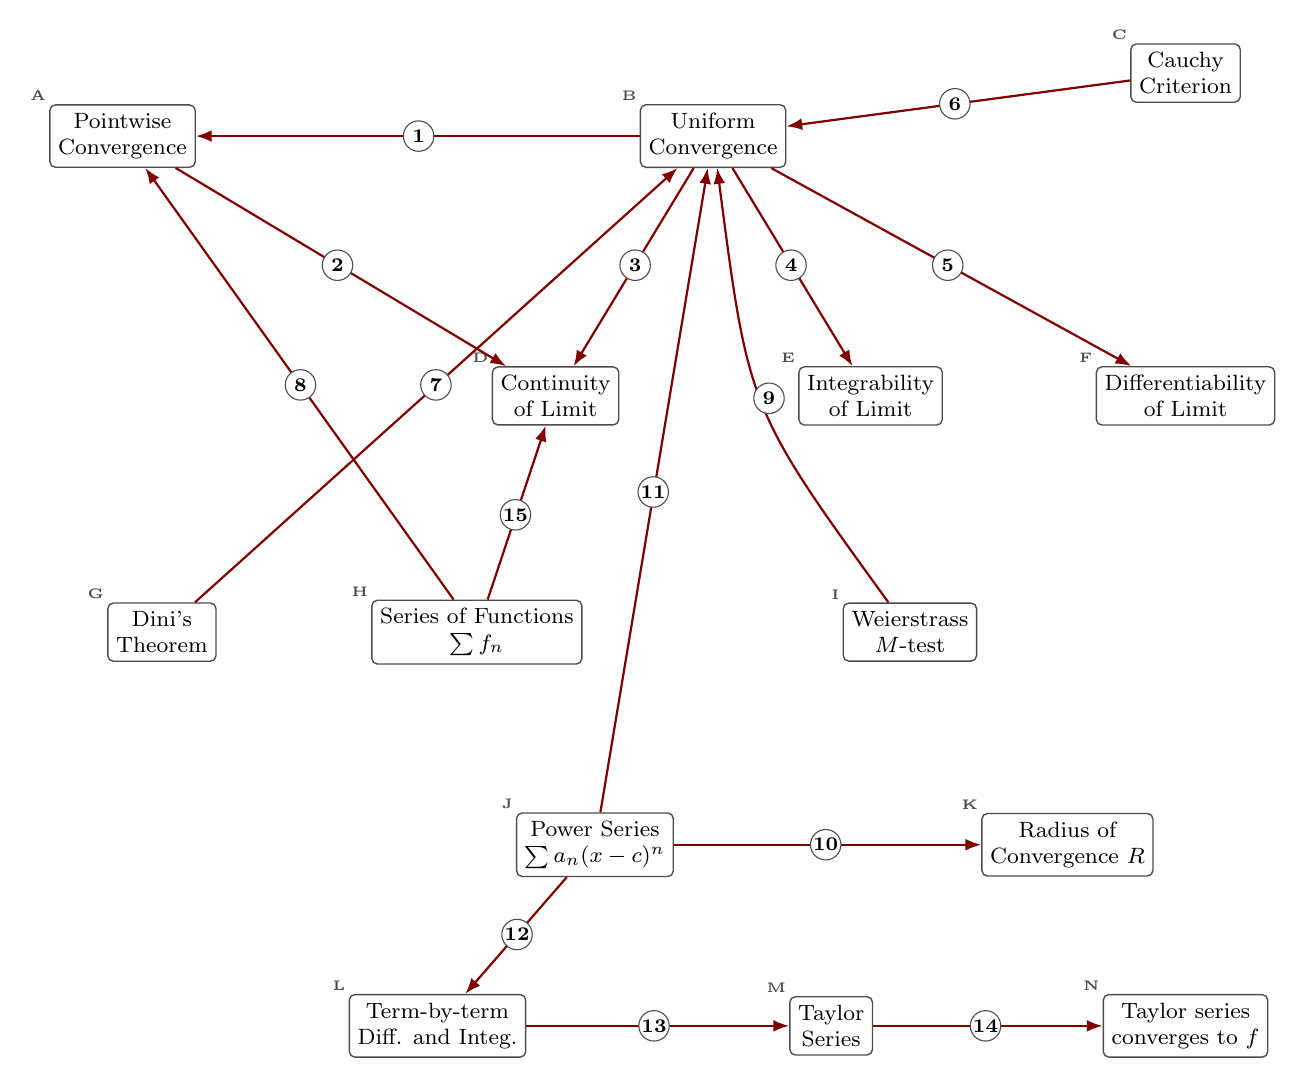
\begin{tikzpicture}[>=Latex]
  \node[concept] (A) at (-6, 0) {Pointwise \\ Convergence};
  \node[concept] (B) at (1.5, 0) {Uniform \\ Convergence};
  \node[concept] (C) at (7.5, 0.8) {Cauchy \\ Criterion};
  \node[concept] (D) at (-0.5, -3.3) {Continuity \\ of Limit};
  \node[concept] (E) at (3.5, -3.3) {Integrability \\ of Limit};
  \node[concept] (F) at (7.5, -3.3) {Differentiability \\ of Limit};
  \node[concept] (G) at (-5.5, -6.3) {Dini's \\ Theorem};
  \node[concept] (H) at (-1.5, -6.3) {Series of Functions \\ \(\sum f_n\)};
  \node[concept] (I) at (4, -6.3) {Weierstrass \\ \(M\)-test};
  \node[concept] (J) at (0, -9) {Power Series \\ \(\sum a_n(x-c)^n\)};
  \node[concept] (K) at (6, -9) {Radius of \\ Convergence \(R\)};
  \node[concept] (L) at (-2, -11.3) {Term-by-term \\ Diff. and Integ.};
  \node[concept] (M) at (3, -11.3) {Taylor \\ Series};
  \node[concept] (N) at (7.5, -11.3) {Taylor series \\ converges to \(f\)};

  \node[nlabel, anchor=south east] at (A.north west) {A};
  \node[nlabel, anchor=south east] at (B.north west) {B};
  \node[nlabel, anchor=south east] at (C.north west) {C};
  \node[nlabel, anchor=south east] at (D.north west) {D};
  \node[nlabel, anchor=south east] at (E.north west) {E};
  \node[nlabel, anchor=south east] at (F.north west) {F};
  \node[nlabel, anchor=south east] at (G.north west) {G};
  \node[nlabel, anchor=south east] at (H.north west) {H};
  \node[nlabel, anchor=south east] at (I.north west) {I};
  \node[nlabel, anchor=south east] at (J.north west) {J};
  \node[nlabel, anchor=south east] at (K.north west) {K};
  \node[nlabel, anchor=south east] at (L.north west) {L};
  \node[nlabel, anchor=south east] at (M.north west) {M};
  \node[nlabel, anchor=south east] at (N.north west) {N};

  \draw[solved] (B) .. controls (-2.25, 0.00) .. (A);
  \draw[solved] (A) .. controls (-3.25, -1.65) .. (D);
  \draw[solved] (B) .. controls (0.50, -1.65) .. (D);
  \draw[solved] (B) .. controls (2.50, -1.65) .. (E);
  \draw[solved] (B) .. controls (4.50, -1.65) .. (F);
  \draw[solved] (C) .. controls (4.50, 0.40) .. (B);
  \draw[solved] (G) .. controls (-2.00, -3.15) .. (B);
  \draw[solved] (H) .. controls (-3.75, -3.15) .. (A);
  \draw[solved] (I) .. controls (1.95, -3.47) .. (B);
  \draw[solved] (J) .. controls (3.00, -9.00) .. (K);
  \draw[solved] (J) .. controls (0.75, -4.50) .. (B);
  \draw[solved] (J) .. controls (-1.00, -10.15) .. (L);
  \draw[solved] (L) .. controls (0.50, -11.30) .. (M);
  \draw[solved] (M) .. controls (5.25, -11.30) .. (N);
  \draw[solved] (H) .. controls (-1.00, -4.80) .. (D);

  \node[edgenum] at (-2.24, -0.00) {1};
  \node[edgenum] at (-3.27, -1.64) {2};
  \node[edgenum] at (0.51, -1.64) {3};
  \node[edgenum] at (2.49, -1.64) {4};
  \node[edgenum] at (4.48, -1.64) {5};
  \node[edgenum] at (4.57, 0.41) {6};
  \node[edgenum] at (-2.02, -3.16) {7};
  \node[edgenum] at (-3.74, -3.16) {8};
  \node[edgenum] at (2.21, -3.33) {9};
  \node[edgenum] at (2.93, -9.00) {10};
  \node[edgenum] at (0.74, -4.52) {11};
  \node[edgenum] at (-0.99, -10.14) {12};
  \node[edgenum] at (0.75, -11.30) {13};
  \node[edgenum] at (4.96, -11.30) {14};
  \node[edgenum] at (-1.01, -4.81) {15};
\end{tikzpicture}
\end{center}
\vspace*{\fill}
\newpage
\heading{The arrows}
\small
\begin{multicols}{2}
\begin{enumerate}[label=\textbf{\arabic*.}, itemsep=0.55em, leftmargin=1.8em]
\item
  {\scriptsize\bfseries\color{maroon} holds.}\ Uniform convergence is pointwise convergence with an \(N\) that does not depend on \(x\), so it is the stronger of the two.
\item
  {\scriptsize\bfseries\color{maroon} fails.}\ Pointwise convergence does not carry continuity to the limit, and \(x^n\) on \([0,1]\) is the witness.
\item
  {\scriptsize\bfseries\color{maroon} holds.}\ A uniform limit of continuous functions is continuous.
\item
  {\scriptsize\bfseries\color{maroon} holds.}\ A uniform limit of integrable functions is integrable, and the limit of the integrals is the integral of the limit.
\item
  {\scriptsize\bfseries\color{maroon} other hypotheses.}\ For the derivative to pass to the limit it is the derivatives that must converge uniformly, and uniform convergence of the functions themselves is not enough.
\item
  {\scriptsize\bfseries\color{maroon} equivalent.}\ A sequence of functions converges uniformly exactly when it is uniformly Cauchy, so neither statement needs the limit named in advance.
\item
  {\scriptsize\bfseries\color{maroon} holds.}\ On a closed bounded interval, monotone pointwise convergence of continuous functions to a continuous limit is already uniform.
\item
  {\scriptsize\bfseries\color{maroon} holds.}\ A series of functions is the sequence of its partial sums, so every statement about sequences of functions applies to it unchanged.
\item
  {\scriptsize\bfseries\color{maroon} holds.}\ Bounding each term by a constant whose series converges gives uniform and absolute convergence of the series of functions.
\item
  {\scriptsize\bfseries\color{maroon} holds.}\ A power series converges absolutely inside one radius and diverges outside it, and that radius is what the ratio or root test computes.
\item
  {\scriptsize\bfseries\color{maroon} holds.}\ Inside its radius a power series converges uniformly on every closed bounded subinterval, which is what licenses working on it term by term.
\item
  {\scriptsize\bfseries\color{maroon} holds.}\ Because the convergence is uniform on compact subintervals, a power series can be differentiated and integrated term by term, and the result keeps the same radius.
\item
  {\scriptsize\bfseries\color{maroon} holds.}\ Differentiating term by term at the centre forces the coefficients to be \(f^{(n)}(c)/n!\), so a function has at most one power series about a point.
\item
  {\scriptsize\bfseries\color{maroon} holds.}\ The Taylor series converges to \(f\) at a point exactly when the remainder tends to zero there, which is a statement about \(f\) and not about the coefficients.
\item
  {\scriptsize\bfseries\color{maroon} holds.}\ Applying the interchange theorems to the partial sums gives the matching statements for the sum of a series of functions.
\end{enumerate}
\end{multicols}
\normalsize
\heading{One last question}
Which single arrow carries the most of this chapter? Say why in one sentence. If your answer is the one arrow whose hypotheses are not what you expected, say what you expected instead.

\vfill
{\scriptsize\color{inkgrey} Contents by Subhadip Chowdhury, licensed CC BY-NC-SA 4.0. Built with AI assistance; the mathematics was checked by a human.\par}
\end{document}
